\section{Animation}

\paragraph{Einstellungsparameter:}

\begin{itemize}
    \item Beschleunigungsspannung $U_B$ im Bereich von 12 kV bis 16 kV und  zugehöriger Richtungsvektor $\vv{s} = \vektor{1}{0}{0}$ der Beschleunigungsstrecke.
    \item Magnetfeldstärke zweier Ablenkspulen:
    
    \begin{itemize}
        \item $B_1$ im Bereich -5 mT bis 5 mT, zugehöriger Richtungsvektor $\vv{b_1} = \vektor{0}{0}{1}$ % senkrechte Spule
        \item $B_2$ im Bereich -5 mT bis 5 mT, zugehöriger Richtungsvektor $\vv{b_2} = \vektor{0}{1}{0}$ % waagerechte Spule
    \end{itemize}

\end{itemize}

\paragraph{Konstanten:}

\begin{itemize}
    \item Felddurchmesser $d$ = 30 in mm
    \item Masse des Elektrons $m$ =  $9,109 \cdot 10^{-31}$ in kg
    \item Ladung des Elektrons $e$ = $1,602 \cdot 10^{-19}$ in As
    \item Bildschirmabstand $l$ = 500 in mm
\end{itemize}

\paragraph{meine zu berechnenden Parameter:}

\begin{itemize}
    \item Teilchengeschwindigkeit v in $\frac{km}{s}$
    \item Ergebnisvektor $\vv{v}$
    \item Bahnradius r in mm 
    \item alpha $\alpha$
    \item Ablenkungsrichtung $\vv{a}$
\end{itemize}

\section{Berechnungen zur Elektronenkanone}

\subsection{physikalische Erklärung:}

 
Ein Netzgerät liefert die Heizspannung, die Spannung für die Bündelung des Elektronenstrahls sowie die Anodenspannung für die Beschleunigung der Elektronen.
Durch die Heizung wird die Kathode zum Glühen gebracht, wodurch Elektronen aus der Kathode austreten (glühelektrischer Effekt), wobei die Elektronen zu Beginn eine Geschwindigkeit von fast $0$ haben.
Im homogenen elektrischen Feld zwischen Kathode (negativ) und Anode (positiv) werden die Elektronen beschleunigt.
Dadurch fliegen Sie mit zunehmender Geschwindigkeit auf die Anode zu.
Dahin werden die Elektronen durch einen Wehnelt-Zylinder auf der Mittelachse konzentriert.
Wegen dieser Richtungsfokussierung sowie ihrer erreichten Geschwindigkeit "`fliegen"' die Elektronen durch die Annodenbohrung hindurch und kommen als gebündelter und gradlinig bewegender Elektronenstrahl aus der Elektronenkanone hinaus.
$$ E_{kin} = E_{el}$$
$$ \frac{1}{2} \cdot m \cdot v^2 = e \cdot U_B$$
Diese Formel wird  nun nach v umgestellt:
%\subsection{Die physikalische Formel:} 
\begin{equation}
\label{eq:v}
   v = \sqrt{\frac{2 \cdot e \cdot U_B}{m}} 
\end{equation}
$$ $$

\subsection{Erklärung/Umsetzung der Physik im Code:}

Im Folgenden ist der Code in der Simulation dargestellt.
Zu sehen ist, dass die oben genannte Formel benutzt wird und die jeweiligen Attribute aus den zugehörigen Klassen geholt werden.
Hier muss sich die Spannung $U_B$ aus der Elektronenkanone (\lstinline$quelle$)  geholt werden.
Des Weiteren wird die Spannung mit 1000 multipliziert, da in der Formel mit Volt gerechnet wird, während die Spannung der Elektronenkanone in Kilovolt angegeben ist. Deswegen muss diese noch umgerechnet werden.

\begin{lstlisting}
teilchengeschwindigkeit 
  = Math.sqrt(2 
  * elektronenladung 
  * quelle.spannung 
  * 1000 
  / elektronenmasse);
\end{lstlisting}

\section{Lorentzkraft und Ablenkung}

\subsection{physikalische Erklärung:}

Das Magnetfeld der Ablenkspulenpaare ist homogen und steht senkrecht zu der Bewegungsrichtung der Elektronen.
Die Elektronen kommen mit einer gewissen Geschwindigkeit $v$ aus der Elektronenkanone heraus und diese bleibt auch im weiteren Verlauf konstant.
Dies bedeutet, dass die Lorentzkraft $F_L$ stets senkrecht zur Bewegungsrichtung der Elektronen wirkt und ihr Betrag dadurch konstant bleibt.
Dies bedeutet, dass Sie deswegen als Zentripetalkraft auf die Elektronen wirkt und diese dadurch auf eine Kreisbahn zwingt.
Wie bereits beschrieben, wirkt die Lorentzkraft als Zentripetalkraft immer senkrecht auf die Bewegungsrichtung der Elektronen.
Dies bedeutet, dass die Kraftkomponente in Bewegungsrichtung nicht vorhanden ist und die Geschwindigkeit deswegen konstant bleibt.
Dadurch leitet sich ab: 
$$ F_L=F_z$$
$$ e \cdot v \cdot B = \frac{m \cdot v^2}{r}$$
Dies lässt sich nun nach $r$ umstellen und man erhält die Formel \ref{eq:r}.   

%\subsection{Die physikalische Formel:}

\begin{equation}
     \label{eq:r}
     r = \frac{m \cdot v}{e \cdot B}
\end{equation}

\section{Geometrische Bestimmung des Winkels}

\subsection{geometrische Erklärung:}

Um geometrisch die Ablenkung zu berechnen muss die Annahme getroffen werden, dass die Ablenkung des Magnetfeldes nur in einem kreisförmigen Ausschnitt wirkt.
Die Situation ist wie in der Skizze in der Abbildung \ref{fig:ausBlog} dargestellt.\cite{Blog}
Aus der Skizze ergibt sich, dass der Ablenkwinkel, um den der Strahl geknickt wird, gleich ist zu dem Winkel im großen Kreis zwischen den Punkten A (Eintrittspunkt in den kleinen Kreis) und B (Austrittspunkt aus dem kleinen Kreis).
Im rechtwinkligen Dreieck aus dem Punkt A und den beiden Mittelpunkten der Kreise, kann man die Definition des Tangens benutzen.
Der Winkel ist $\frac{\alpha}{2}$ da die Winkelhalbierende als Verbindungslinie fungiert.
Also gilt die Formel \ref{eq:tan}.
Um festzustellen in welche Richtung um den Winkel $\alpha$ abgelenkt wird, müssen die Richtungsvektoren des Strahls und des Magnetfeldes betrachtet werden.
Die Lorentzkraft wirkt in die Richtung des Kreuzprodukts dieser beiden.
Da mit negativen Teilchen gearbeitet wird, muss der Richtungsvektor des Strahls umgedreht werden. Dadurch ergibt sich die Formel \ref{eq:a}.
Um den Endpunkt auf dem Schirm zu bestimmen, kann sich die Skizze wie in Abbildung \ref{fig:Schirm} dargestellt, zu Hilfe genommen werden.
Der Punkt M stellt den Mittelpunkt des kleinen Kreises aus der Abbildung \ref{fig:ausBlog} da.
Der Punkt E stellt den Punkt da, wo der Strahl auf den Schirm trifft. Der Punkt U hingegen stellt den Mittelpunkt des Schirm da.
Der Winkel $\alpha$ stellt den Winkel da, welcher mit der Formel \ref{eq:tan} da und $\vv{a}$ stellt die Ablenkrichtung des Strahl da, welche mit der Formel \ref{eq:a} berechnet wurde.
Da man ein rechtwinkliges Dreieck hat kann man die Länge ausrechnen, welche die Seite $\vv{UE}$ hat.
Dies entspricht $\vv{v_{diff}}$.
Man erhält einen Vektor welchen man auf U draufaddieren kann.
Dadurch erhält man die Formel \ref{eq:v}.
Da mit zwei Magneten gearbeitet wird, müssen die Formeln \ref{eq:tan}, \ref{eq:a} und \ref{eq:v} jeweils zweimal gemacht werden.
Nun ist der Vektor $\vv{v_{diff}}$ zweimal vorhanden, einmal für das senkrechte und einmal für das waagerechte Magnetfeld, diese beide Vektoren werden nun auf den Punkt U draufaddiert, sodass der Punkt E erhalten wird.
\begin{figure}
    \centering
    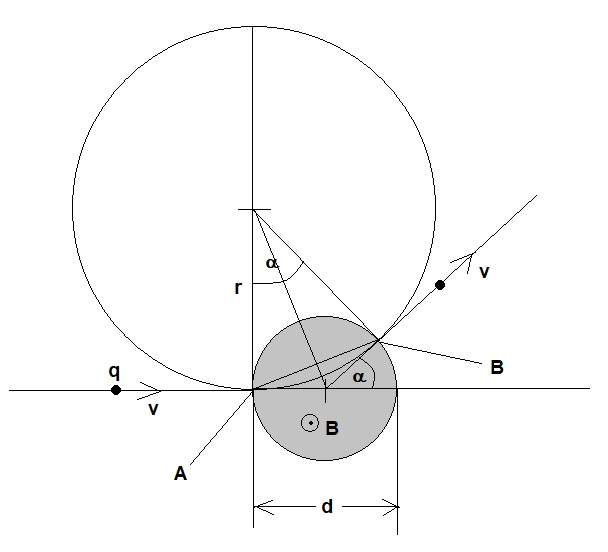
\includegraphics[width=.75\textwidth]{fig/elektronenstrahl-ablenkung_101.jpg}
    \caption{Skizze für Winkelberechnung}
    \label{fig:ausBlog}
\end{figure}

\begin{figure}
    \centering
    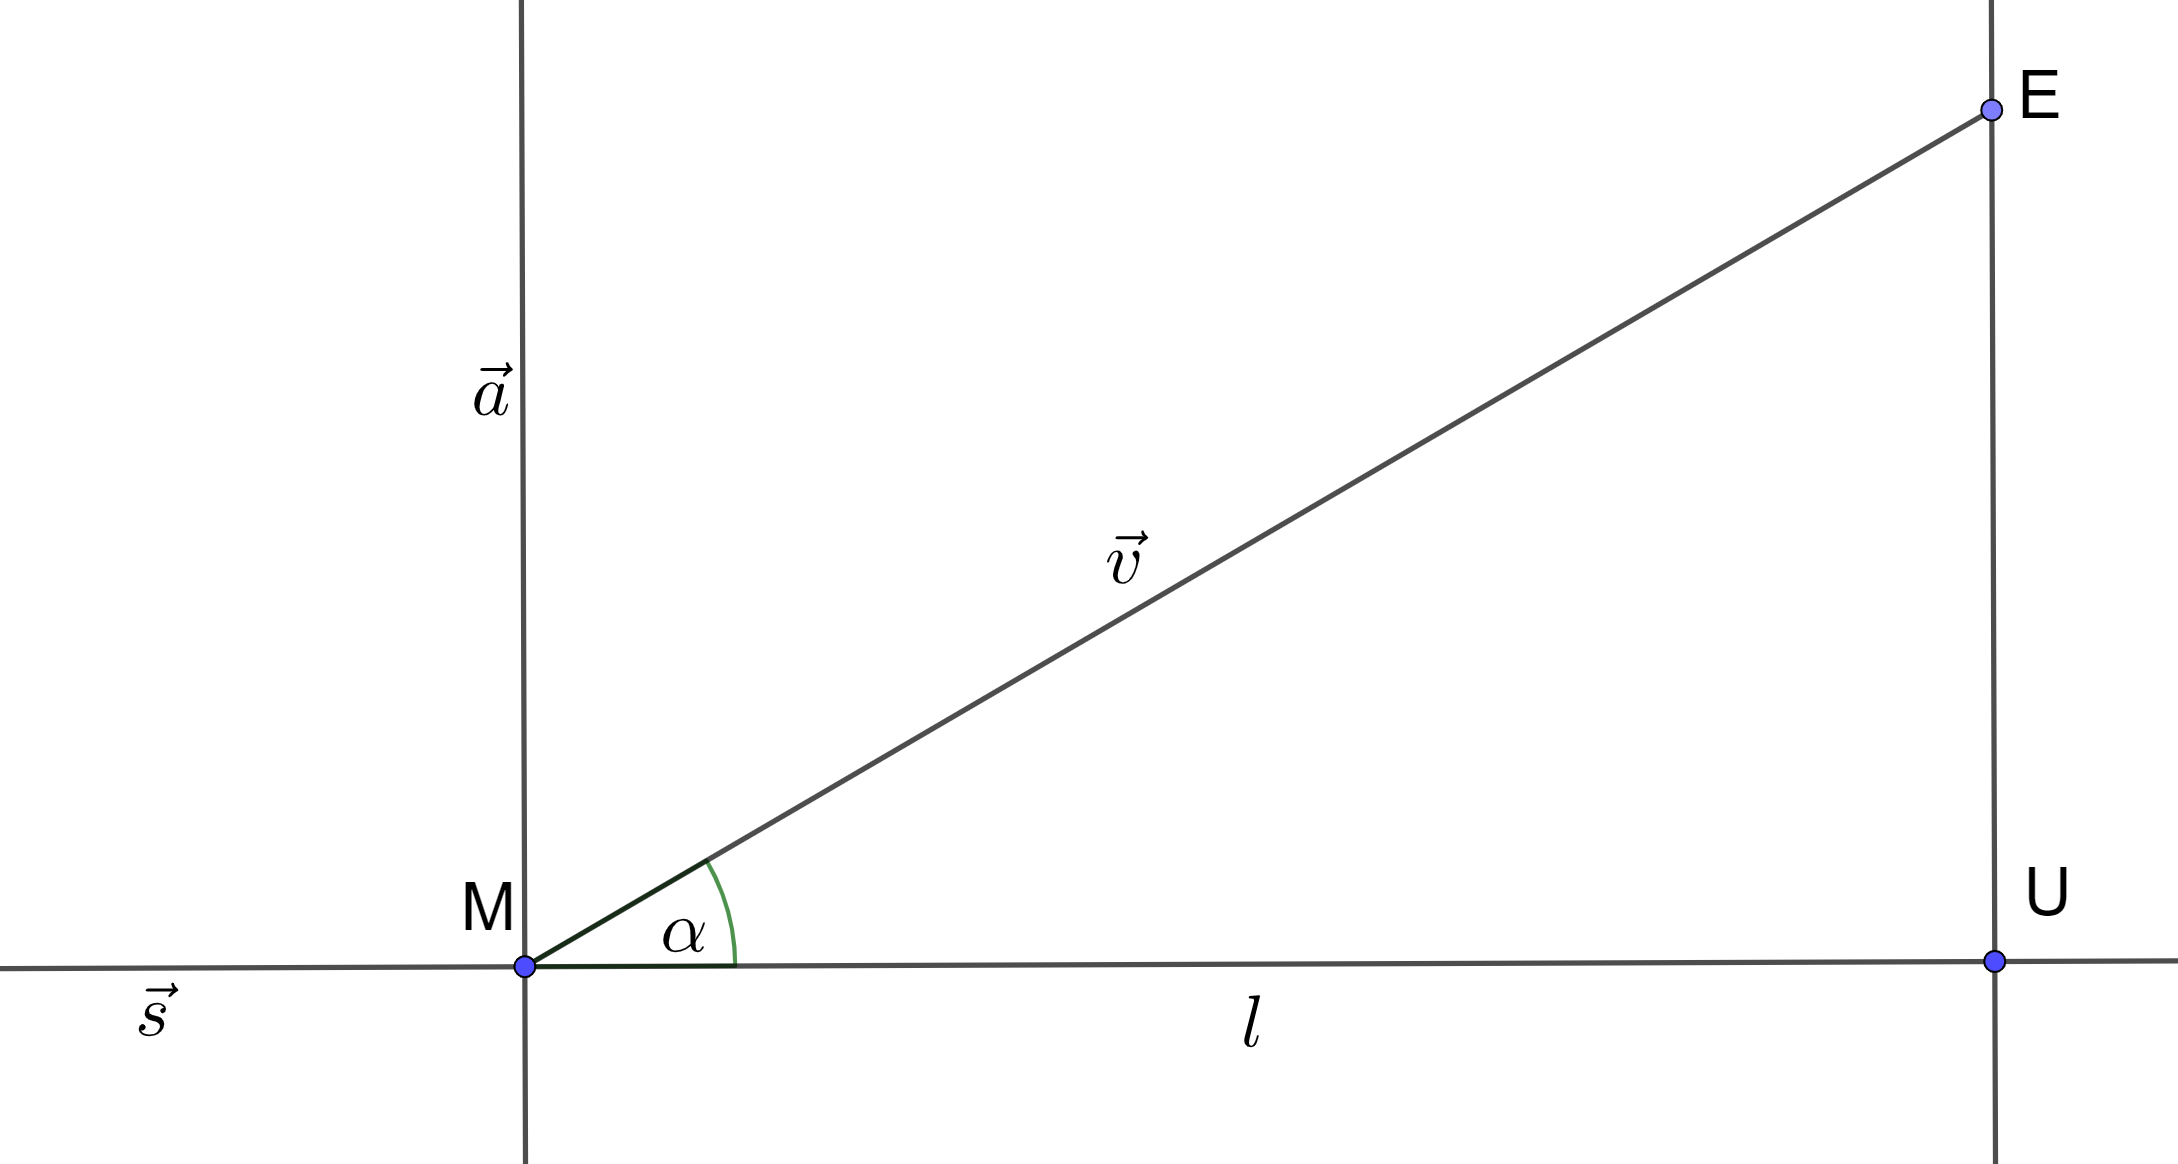
\includegraphics[width=.75\textwidth]{fig/Bildschirm_Skizze.png}
    \caption{Skizze für Auftreffen auf Bildschirm}
    \label{fig:Schirm}
\end{figure}

%\subsection{Die geometrische Formel:}
\begin{equation}
    \label{eq:tan}
    \tan(\frac{\alpha}{2}) = \frac{d}{2}:r = \frac{d}{2 \cdot r}
\end{equation}

\begin{equation}
    \label{eq:a}
    \vv{a} = \vv{s} \cdot (-1) \times \vv{b}
\end{equation}

\begin{equation}
    \label{eq:v}
    \vv{v_{diff}} =  \vv{a} \cdot l \cdot \tan(\alpha)
\end{equation}

\subsection{Erklärung/Umsetzung der Physik im Code:}

Bei der Berechnung des Winkels $\alpha$ wird der arctans der oben bereits genannte Formel \ref{eq:tan} genommen und mit zwei multipliziert, da auf der Ausgabe der tatsächliche Winkel $\alpha$ zu sehen sein soll.
Des Winkel $\alpha$ wird im Bogenmaß berechnet.
Bei der \lstinline$Ablenkungsrichtung$ wird der Richtungsvektor des Strahl mit $-1$ multipliziert und danach das Kreuzprodukt mit dem Richtungsvektor des Ablenkspulenpaars genommen, wie bereits in Formel \ref{eq:a} genannt.
Durch den Befehl \lstinline$this.richtungsvektor$ wird auf den Richtungsvektor des jeweiligen Magnetes verwiesen.
Des Weiteren ist noch hinzuzufügen, dass die Berechnung jedes Ablenkspulenpaar für sich macht uns daher auch eigene Werte für \lstinline$alpha$, den \lstinline$Bahnradius$ und die \lstinline$Ablenkungsrichtung$ hat.
Der \lstinline$Ergebnisvektor$ ist ein Vektor der gespeichert wird und später dafür verwendet wird, dass der Strahl vom Magneten zu dem Vektor auf dem Bildschirm gezeichnet wird.
Durch den \lstinline$for$ Befehl wird bewirkt, dass wie oben bereits genannt die Berechnung des \lstinline$Ergebnisvektors$ für jeden der Magneten gemacht werden muss.
Dies bedeutet, dass der \lstinline$Ergebnisvektor$, welcher zu Beginn auf den \lstinline$bildschirmabstand$ als x- Koordinate, $0$ als y-Koordinate und 0 als z-Koordinate gesetzt ist, erst die Formel \ref{eq:v} benutzt wird und addiert wird.
Danach wird die Formel \ref{eq:v} erneut benutzt und erneut addiert. Dies führt dazu, dass der Punkt auf dem Schirm E nun berechnet ist.

\begin{lstlisting}
alpha = 2 * Math.atan(felddurchmesser/ (2 *bahnradius ));
ablenkungsrichtung
  = strahl.quelle.richtungsvektor.
    multiplizieren(-1).
    kreuzprodukt(this.richtungsvektor);

Vektor ergebnisvektor = new Vektor(bildschirmabstand,0,0);
    for(Ablenkspulenpaar m : getWorld().getObjects(Ablenkspulenpaar.class) )
    {
        ergebnisvektor 
        = ergebnisvektor.addieren( m.ablenkungsrichtung.
        multiplizieren(bildschirmabstand*Math.tan(m.alpha)));
    }
return ergebnisvektor;

\end{lstlisting}

%\begin{tabular}{c|c|c}
    % Formel Buch & Formel Block & Anmerkungen  \\
     %\hline
    %$\alpha = \frac{d}{r}$ &$\tan(\frac{\alpha}{2}) = \frac{d}{2\cdot r}$& wegen Kleinwinkelnäherung bei dem Buch \\
    %\hline
   %$r = \frac{m\cdot v}{q\cdot B}$  & $r = \frac{m\cdot v}{q\cdot B}$& alles gleich 
     
%\end{tabular}
